\documentclass[Ligatures=TeX,table,brazil,svgnames,usetotalslideindicator,compress,10pt]{beamer}

\usetheme[titleformat=allsmallcaps]{metropolis}

\usepackage{polyglossia}
\setdefaultlanguage{brazil}
\disablehyphenation

\usepackage{minted}

\usetikzlibrary{arrows,positioning,calc}

\usepackage{graphicx}
\graphicspath{{./figuras/}}
\usepackage{subcaption}
\usepackage{xmpmulti}

% \usepackage{textpos}

% \usepackage{mdwlist}
% \usepackage{siunitx}
\usepackage{alltt}
% \usepackage{multicol}
\usepackage{xspace}
\usepackage{multirow}
\usepackage{amsmath}

\usepackage{cancel}
\usepackage{fontawesome}

\newcommand{\setcoverbg}{
  \setbeamertemplate{background}
  {\includegraphics[width=\paperwidth,height=\paperheight]{backgrounds/coverbg}}
}
\newcommand{\setintersectionbg}{
  \setbeamertemplate{background}
  {\includegraphics[width=\paperwidth,height=\paperheight]{backgrounds/blank}}
}
\newcommand{\setsectionbg}{
  \setbeamertemplate{background}
  {\includegraphics[width=\paperwidth,height=\paperheight]{backgrounds/slidebg2}}
}

\setbeamertemplate{caption}{default}

\title{MCTA025-13 - Sistemas Distribuídos}
\subtitle{Replicação e Consistência}

\author{Emilio Francesquini}
\institute{Centro de Matemática, Computação e Cognição\\ Universidade Federal do ABC}
\date{13 e 15 de agosto de 2018}

\begin{document}

\setcoverbg
\maketitle

\setsectionbg

\begin{frame}
  \frametitle{Disclaimer}
  \begin{itemize}
  \item Estes slides foram preparados para o curso de \textbf{Sistemas
      Distribuídos na UFABC}.
  \item Este material pode ser usado livremente desde que sejam
    mantidos, além deste aviso, os créditos aos autores e
    instituições.
  \item Estes slides foram adaptados daqueles originalmente preparados
    (e gentilmente cedidos) pelo professor \textbf{Daniel Cordeiro, da
      EACH-USP} que por sua vez foram baseados naqueles
    disponibilizados online pelos autores do livro ``Distributed
    Systems'', 3ª Edição em:
    \url{https://www.distributed-systems.net}.
  \end{itemize}
\end{frame}


\begin{frame}
  \frametitle{Consistência \& Replicação}
  \begin{itemize}
  \item Introdução (do que se trata isso?)
  \item Consistência centrada nos dados
  \item Consistência centrada no cliente
  \item Gerenciamento de réplicas
  \item Protocolos de consistência
  \end{itemize}
\end{frame}

\begin{frame}
  \frametitle{Desempenho e escalabilidade}
  \begin{block}{Problema principal}
    Para manter a consistência entre as réplicas, geralmente
    precisamos garantir que todas as operações \textbf{conflitantes}
    sejam realizadas na mesma ordem em todas as réplicas
  \end{block}

  \begin{block}{Operações conflitantes}
    Terminologia da área de controle de transações:
    \begin{description}
    \item[read--write] conflito onde uma operação de leitura e uma de escrita ocorrem de forma concorrente
    \item[write--write] conflito com duas operações concorrentes de escrita
    \end{description}
  \end{block}

  \begin{block}{Problema}
    Garantir a ordem global de operações conflitantes pode ser muito
    custoso, diminuindo a escalabilidade. \alert{Solução:} diminuir os
    requisitos de consistência e, com sorte, conseguir evitar
    sincronizações globais
  \end{block}

\end{frame}

\section{Modelos de consistência centrados em dados}

\begin{frame}
  \frametitle{Modelos de consistência centrados em dados}

  \begin{block}{Modelo de consistência}
    É um contrato entre um \textit{data store} (armazém de dados) distribuído e os processos, no qual o \textit{data store} define precisamente o resultado de operações concorrentes de leitura e escrita
  \end{block}

  \begin{alertblock}{Importante:}
    Um \textit{data store} é uma coleção de dispositivos de armazenamento distribuídos
    \begin{figure}
      \centering
      \includegraphics[width=.7\textwidth]{07-01}
    \end{figure}
  \end{alertblock}

\end{frame}

\begin{frame}
  \frametitle{Consistência contínua}
  \begin{block}{Observação}
    Podemos considerar diferentes \textbf{graus de consistência}:
    \begin{itemize}
    \item réplicas podem diferir em relação aos seus \textbf{valores numéricos}
    \item réplicas podem diferir em relação à \textbf{desatualização relativa}
    \item pode haver diferenças no número e na ordem das \textbf{operações de atualizações realizadas}
    \end{itemize}
  \end{block}

  \begin{alertblock}{Conit: consistency unit}
    Especifica a \alert{unidade de dados} sob a qual a consistência será medida
  \end{alertblock}

\end{frame}

\begin{frame}
  \frametitle{Exemplo: Conit}
  \begin{figure}
    \centering
    \includegraphics[width=.7\textwidth]{07-02}
  \end{figure}
  \begin{block}{Conit: variáveis d, g e p}
    \begin{itemize}
    \item Cada réplica possui um \textbf{relógio vetorial}: \mbox{\alert{(tempo conhecido @ A, tempo conhecido @ B)}}
    \item $B$ envia à $A$ a operação [$\langle 5,B \rangle$: $g \leftarrow g + 45$]; $A$ faz com que a operação se torne \alert{permanente} (não pode ser \textit{rolled back})
    \end{itemize}
  \end{block}

\end{frame}

\begin{frame}
  \frametitle{Exemplo: Conit}
  \begin{figure}
    \centering
    \includegraphics[width=.7\textwidth]{07-02}
  \end{figure}
  \begin{block}{Conit: variáveis d, g e p}
    \begin{itemize}
      \item $A$ tem três operações \textbf{pendentes} (desvio de ordem = 3)
      \item $A$ perdeu \textbf{duas} operações de $B$, resultando em uma diferença máxima de 70+412 unidades $\Rightarrow$ $(2,482)$ (desvio numérico)
    \end{itemize}
  \end{block}

\end{frame}

\begin{frame}
  \frametitle{Consistência sequencial}

  \begin{block}{Definição}
    O resultado de qualquer execução é o mesmo, como se as operações de
    todos os processos fossem executadas na mesma ordem sequencial e as
    operações de cada processo aparecer nessa sequência na ordem
    especificada pelo seu programa.
  \end{block}

  \begin{figure}
  \begin{tabular}{cc}
    \includegraphics{07-05a} &
    \includegraphics{07-05b}
  \end{tabular}
\end{figure}

(a) é um \textit{data store} com consistência sequencial; (b) não apresenta consistência sequencial

\end{frame}

\begin{frame}
  \frametitle{Consistência Sequencial --- Exemplo}
  \begin{table}[]
    \begin{tabular}{lll}
      \textbf{Processo 1} & \textbf{Processo 2} & \textbf{Processo 3} \\ \hline
      \texttt{x = 1;}               & \texttt{Y = 1;}       & \texttt{Z = 1;}\\
      \texttt{print(Y, Z);}         & \texttt{print(X, Z);} & \texttt{print(X, Y);}

    \end{tabular}
  \end{table}
  \pause
  \begin{itemize}
  \item \textbf{6!} combinações possíveis\ldots
  \item<3-> \ldots mas são todas \alert{válidas}?
  \end{itemize}

\end{frame}


\begin{frame}
  \frametitle{Consistência Sequencial --- Exemplo}
  \begin{figure}
    \includegraphics[width=1.1\textwidth]{seq_cons_a}
  \end{figure}
  \begin{itemize}
  \pause
  \item A assinatura \alert{\texttt{00 00 00}} é válida?
  \pause
  \item A assinatura \alert{\texttt{00 10 01}} é válida?
  \end{itemize}
\end{frame}



\begin{frame}
  \frametitle{Consistência causal}
  \begin{block}{Definição}
    Operações de escrita que potencialmente possuem uma relação de causalidade devem ser vistas por todos os processos na mesma ordem. Escritas concorrentes podem ser vistas em uma ordem diferente por processos diferentes.
  \end{block}

  \begin{figure}
    \centering
    \includegraphics[scale=0.9]{07-09}
  \end{figure}

  \small
  (a) uma violação da consistência causal; (b) uma sequência correta de eventos em um \textit{data store} com consistência causal

\end{frame}

\begin{frame}
  \frametitle{Compatibilidade Sequencial-Causal}
  \begin{figure}[ht]
    \centering
    \includegraphics{07-10-new}
  \end{figure}
  \begin{itemize}
  \item É \textbf{sequencialmente} consistente?
  \item É \textbf{causalmente} consistente?
  \end{itemize}
\end{frame}


\begin{frame}
  \frametitle{Agrupamento de operações}
  \begin{block}{Definição}
    \begin{itemize}
    \item acessos às \alert{variáveis de sincronização} (\textit{locks}) possuem consistência sequencial
    \item o acesso às variáveis de sincronização não é permitido até que todas as escritas anteriores tenham terminado em todos os lugares
    \item nenhum acesso aos dados é permitido até que todos os acessos às variáveis de sincronização tenham sido feitos
    \end{itemize}
  \end{block}

  \begin{block}{Ideia básica:}
    Você não precisa se preocupar se as leituras e escritas de uma
    \textbf{série} de operações serão imediatamente do conhecimento de
    todos os processos. Você só quer que o \textbf{efeito} dessa série
    seja conhecido.
  \end{block}
\end{frame}

\begin{frame}
  \frametitle{Argupamento de operações}

  \begin{figure}
    \centering
    \includegraphics{07-10}
    \caption{Um sequência de eventos que respeita a consistência de entrada.}
  \end{figure}


  \begin{block}{Observação}
    Consistência de entrada implica a necessidade de proteger os dados
    com \textit{locks} (implícitos ou não)
  \end{block}

\end{frame}

\begin{frame}
  \frametitle{Eventual Consistency}
  \begin{itemize}
  \item Dependendo da aplicação não é problema que as \textbf{atualizações não
    sejam propagadas imediatamente}
    \begin{itemize}
    \item Normalmente os clientes acessam a mesma réplica, então não
      há problemas de inconsistência (na visão do cliente)
    \end{itemize}
  \item Permite uma implementação de \textbf{modelo de consistência com menos
    restrições e portanto mais eficiente} (PQ?)
  \item Exemplos:
    \begin{itemize}
    \item Facebook
    \item DNS
    \item Páginas Web em Geral
    \end{itemize}
  \end{itemize}

\end{frame}

\begin{frame}
  \frametitle{Uma nota sobre \emph{eventual consistency}}
  \begin{block}{\alert{\textbf{EVENTUAL (EN)} $\neq$ \textbf{EVENTUAL (PT)}}}
      O mesmo vale para espanhol, francês, \ldots
    \begin{itemize}
    \item \textbf{eventual (en)} \emph{adjective}: happening at some
      indefinite future time or after a series of occurrences; ultimate

    \item \textbf{eventual (pt)} \emph{a2g}: 1. Que é incerto, podendo
      acontecer ou deixar de acontecer; CASUAL; FORTUITO. 2. Que ocorre
      de vez em quando; OCASIONAL: Tínhamos encontros eventuais. [
      Antôn.: frequente. ]
    \end{itemize}
  \end{block}

  \textbf{\alert{NÃO ESCREVA}} ``consistência eventual'' na prova sob
  risco de causar revolta no seu professor.
  \begin{itemize}
  \item E você \underline{não quer} o seu professor revoltado enquanto ele corrige sua prova.~\faSmileO
  \end{itemize}
  \textbf{Prefira} consistência diferida, consistência postergada, ou até mesmo o termo em inglês ``\emph{eventual consistency}''

\end{frame}


\begin{frame}
  \frametitle{Modelos de consistência centrados no cliente}
  \begin{itemize}
  \item Modelo do sistema
  \item Leituras monotônicas
  \item Escritas monotônicas
  \item \textit{Read-your-writes} (leia-suas-escritas)
  \item \textit{Write-follows-reads} (escrita-segue-leituras)
  \end{itemize}

  \begin{block}{Objetivo}
    Mostrar que talvez manter a consistência em todo o sistema seja
    desnecessário se nos concentramos no que os \textbf{clientes}
    precisam, ao invés daquilo que deve ser mantido pelos servidores.
  \end{block}
\end{frame}

\begin{frame}
  \frametitle{Consistência para usuários móveis}
  \begin{exampleblock}{Exemplo}
    Considere um sistema de banco de dados distribuídos no qual você tem acesso pelo seu notebook. Assuma que seu notebook seja o \textit{front end} do seu banco de dados.
  \end{exampleblock}

  \begin{itemize}
  \item no local $A$ você acessa o banco de dados e realiza leituras e atualizações
  \item no local $B$ você continua seu trabalho, mas, a não ser que você continue acessando o mesmo servidor de antes, você poderá detectar algumas inconsistências:
    \begin{itemize}
    \item suas atualizações em $A$ podem ainda não terem sido propagadas para $B$
    \item você pode estar lendo entradas mais novas do que aquelas disponíveis em $A$
    \item suas atualizações em $B$ podem eventualmente conflitar com aquelas em $A$
    \end{itemize}
  \end{itemize}

\end{frame}

\begin{frame}
  \frametitle{Consistência para usuários móveis}
  \begin{alertblock}{Observação}
    A única coisa que você realmente precisa é que as entradas que você atualizou e/ou leu em $A$ estejam em $B$ do modo que você as deixou em $A$. Nesse caso, o banco de dados parecerá consistente \textbf{para você}
  \end{alertblock}
\end{frame}

\begin{frame}
  \frametitle{Arquitetura básica}
  \begin{figure}
    \centering
    \includegraphics[width=\textwidth]{07-11}
  \end{figure}
\end{frame}

\begin{frame}
  \frametitle{Leituras monotônicas}
  \begin{block}{Definição}
    Se um processo ler o valor de um item $x$, quaisquer leituras sucessivas de $x$ feitas por esse processo sempre devolverão o mesmo valor ou um valor mais recente.
  \end{block}

  \begin{figure}
    \centering
    \includegraphics{07-12}
  \end{figure}

  \small
  Leituras realizadas por um processo $P$ em duas cópias locais diferentes do mesmo \textit{data store}. (a) Uma leitura monotônica consistente; (b) um \textit{data store} que não provê leituras monotônicas

\end{frame}

\begin{frame}
  \frametitle{Consistência centrada no cliente: notação}
  \begin{block}{Notação}
    \begin{itemize}
    \item $W_1(x_2)$ é a operação de escrita feita pelo processo $P_1$ que leva à versão $x_2$ de $x$
    \item $W_1(x_i;x_j)$ indica que $P_1$ produziu a versão $x_j$ baseado na versão anterior $x_i$
    \item $W_1(x_i|x_j)$ indica que $P_1$ produziu a versão $x_j$ \alert{concorrentemente} a versão $x_i$
    \end{itemize}
  \end{block}
\end{frame}

\begin{frame}
  \frametitle{Leituras monotônicas}
  \begin{exampleblock}{Exemplo}
    Leituras automáticas das atualizações em seu calendário pessoal vindas de diferentes servidores. Leituras monotônicas garantem que o usuário veja todas as atualizações, independentemente do servidor que originou a leitura
  \end{exampleblock}

  \pause
  \begin{exampleblock}{Exemplo}
    Ler (sem modificar) as mensagens enquanto você estiver em movimento. Toda vez que você se conectar a um servidor de e-mails diferente, o servidor irá descarregar (pelo menos) todas as atualizações do servidor que você visitou antes
  \end{exampleblock}

\end{frame}

\begin{frame}
  \frametitle{Escritas monotônicas}
  \begin{block}{Definição}
    Uma escrita monotônica feita por um processo em um dado
    $x$ é terminada antes de quaisquer operações de escrita sucessivas
    em $x$ por esse mesmo processo.
  \end{block}

  \begin{figure}
    \centering
    \includegraphics{07-13}
  \end{figure}

  Ou seja, se tivermos duas escritas sucessivas $W_k(x_i)$ e $W_k(x_j)$, então não importa onde $W_k(x_j)$ acontece, sempre teremos $W_k(x_i;x_j)$.

\end{frame}

\begin{frame}
  \frametitle{Escritas monotônicas}

  \begin{exampleblock}{Exemplo}
    Atualizar um programa no servidor $S_2$ e garantir que todos os componentes necessários para a compilação também estejam em $S_2$
  \end{exampleblock}

  \pause
  \begin{exampleblock}{Exemplo}
    Manter versões de arquivos replicados na ordem correta em todos os lugares (propagando as versões antigas para o servidor onde a versão mais nova está instalada)
  \end{exampleblock}

\end{frame}

\begin{frame}
  \frametitle{Read-your-writes}

  \begin{block}{Definição}
    O efeito de uma operação de escrita realizada por um processo no item $x$ sempre será visto por operações de leituras de $x$ pelo mesmo processo.
  \end{block}

  \qquad

  \begin{columns}
    \begin{column}{0.6\textwidth}
      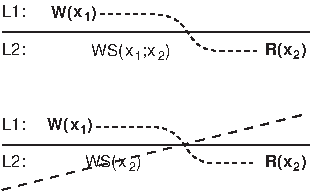
\includegraphics{07-14}
    \end{column}

    \begin{column}{0.4\textwidth}

      \pause
      \begin{exampleblock}{Exemplo}
        Atualizar sua página web e garantir que o navegador web mostre a versão mais nova ao invés de mostrar a versão em cache
      \end{exampleblock}

    \end{column}

  \end{columns}

\end{frame}

\begin{frame}
  \frametitle{Write-follows-read}
  \begin{block}{Definição}
    Uma operação de escrita feita por um processo no item $x$ após uma operação de leitura de $x$ no mesmo processo é garantidamente realizada no mesmo valor de $x$ que foi lido (ou num valor mais novo)
  \end{block}

  \qquad

  \begin{columns}

    \begin{column}{0.6\textwidth}

      \includegraphics{07-15}

    \end{column}

    \begin{column}{0.4\textwidth}

      \pause

      \begin{exampleblock}{Exemplo}
        Ver os comentários a um artigo publicado apenas se você tiver o artigo original (uma leitura ``puxa'' as operações de escrita correspondentes)
      \end{exampleblock}

    \end{column}

  \end{columns}


\end{frame}

\section{Gerenciamento de réplicas}

\begin{frame}
  \frametitle{Protocolos distribuídos}
  \begin{itemize}
  \item posicionamento de servidores de réplicas
  \item replicação de conteúdo e posicionamento
  \item distribuição de conteúdo
  \end{itemize}
\end{frame}

\begin{frame}
  \frametitle{Posicionamento de réplicas}
  \begin{block}{Ideia}
    Encontrar as $K$ melhores posições de uma lista de $N$ possibilidades
  \end{block}

  \begin{itemize}[<+->]
  \item iterativamente selecionar as melhores posições de $N-K$ para as quais a \alert{distância média até os clientes} é mínima e então escolher o próximo melhor servidor (a primeira posição escolhida é a que minimiza a distância média até todos os clientes). \textbf{Computacionalmente caro}
  \item selecionar o $K$-ésimo maior \textbf{sistema autônomo} e colocar um servidor no host ``melhor conectado''. \textbf{Computacionalmente caro}
  \item posicionar os nós em um espaço geométrico $d$-dimensional, onde a distância reflete a latência. Identificar as $K$ regiões mais densas e colocar um servidor em cada uma delas. \textbf{Computacionalmente barato}
  \end{itemize}

\end{frame}

\begin{frame}
  \frametitle{Replicação de conteúdo}
  \begin{block}{Distingue diferentes processos}
    Um processo é capaz de hospedar uma réplica de um objeto ou dado:
  \end{block}
  \begin{itemize}
  \item \textbf{réplicas permanentes:} processo/máquina sempre tem uma réplica
  \item \textbf{réplica iniciada pelo servidor:} processos que podem  hospedar uma réplica dinamicamente, sob demanda de um outro servidor ou \textit{data store}
  \item \textbf{réplica iniciada pelo cliente:} processos que podem hospedar uma réplica dinamicamente, sob demanda de um cliente (\alert{cache do cliente})
  \end{itemize}
\end{frame}

\begin{frame}
  \frametitle{Replicação de conteúdo}

  \includegraphics[width=\textwidth]{07-17}

\end{frame}

\begin{frame}
  \frametitle{Réplicas iniciadas pelo servidor}
  \begin{figure}
    \centering
    \includegraphics{07-18}
  \end{figure}
  \begin{itemize}
  \item mantenha o número de acessos aos arquivos, agregando-os pelo servidor mais próximo aos clientes que requisitarem o arquivo
  \item número de acessos cai abaixo de um threshold $D$ $\Rightarrow$ descartar arquivo
  \item número de acessos acima de um threshold $R$ $\Rightarrow$ replicar arquivo
  \item número de acessos entre $D$ e $R$  $\Rightarrow$ migrar arquivo
  \end{itemize}
\end{frame}

\begin{frame}
  \frametitle{Distribuição de conteúdo}
  \begin{block}{Modelo}
    Considere apenas uma combinação cliente--servidor:
    \begin{itemize}
    \item propaga apenas a \textbf{notificação/invalidação} de uma atualização (normalmente usada por caches)
    \item transfere dados de uma cópia para outra (bancos de dados distribuídos): \alert{replicação passiva}
    \item propaga \textbf{operações} de atualização para outras cópias: \alert{replicação ativa}
    \end{itemize}
  \end{block}

  \begin{alertblock}{Nota}
    Nenhuma abordagem é melhor que outra, seu uso depende da largura de banda disponível e a razão leituras/escritas nas réplicas
  \end{alertblock}
\end{frame}

\begin{frame}
  \frametitle{Distribuição de conteúdo: sistema cliente/servidor}
  \begin{description}
  \item[pushing] \emph{iniciada pelo servidor};  uma atualização é propagada mesmo que o alvo não tenha pedido por ela
  \item[pulling] \emph{iniciada pelo cliente}; uma atualização solicitada pelo cliente
  \end{description}

  \begin{block}{Observação}
    Podemos trocar dinamicamente entre os métodos \textit{pulling} e \textit{pushing} com o uso de \textbf{leases}: um contrato no qual o servidor promete enviar (\textit{push}) atualizações para o cliente até que o \textit{lease} expire.
  \end{block}

\end{frame}

\begin{frame}
  \frametitle{Distribuição de conteúdo}
  \begin{block}{Problema}
    Fazer com que a data de expiração do \textit{lease} dependa do comportamento do sistema (\textit{leases} adaptativos):
    \begin{itemize}
    \item<2,5> \textbf{leases com idade}: um objeto que não for modificado nos últimos tempos não será modificado em um futuro próximo, então conceda um \textit{lease} que dure bastante
    \item<3,5> \textbf{lease baseado na frequência de renovação}: quanto maior a frequência com que o cliente requisitar o objeto, maior a data de expiração para aquele cliente (para aquele objeto)
    \item<4,5> \textbf{lease baseado no estado}: quando mais sobrecarregado o servidor estiver, menor a data da expiração se torna
    \end{itemize}

    \onslide<5-> Por que fazer tudo isso? Para tentar reduzir ao máximo o estado do servidor, mas ainda assim prover consistência forte.
  \end{block}
\end{frame}

\section{Protocolos de consistência}

\begin{frame}
  \frametitle{Protocolos de consistência}
  Descrevem a implementação de um modelo de consistência específico.
  \begin{itemize}
  \item consistência contínua
  \item protocolos \textit{primary-based}
  \item protocolos de replicação de escrita
  \end{itemize}
\end{frame}

\begin{frame}
  \frametitle{Consistência contínua: erros numéricos}
  \begin{block}{Modo de Operação}
    \begin{itemize}

    \item por simplicidade considere apenas um dado, representado por \alert{$x$}

    \item \alert{$W(x)$} representa uma operação de escrita em $x$

    \item \alert{$val(W(x))$} ou simplesmente \alert{$val(W)$}, representa a valor
      (numérico) pelo qual x foi atualizado após a operação de escrita
      $W$. Por simplicidade assuma que \alert{$\forall~W: val(W) > 0$}

    \item cada servidor $S_i$ tem um log de todas as operações de
      escrita denotado por \alert{$L_i$}

    \item $W$ é inicialmente enviado para uma das $N$ réplicas. Essa
      réplica é denotada por \alert{$origin(W)$}.
    \item \alert{$TW[i,j]$} é o resultado (o valor de $x$) das \emph{escritas
        executadas pelo servidor $S_i$ em $x$ que originaram de
        $S_j$}:
        \[TW[i,j] = \sum \{ val(W) | origin(W) = S_j \wedge  W \in L_i \}\]
    \end{itemize}
  \end{block}
\end{frame}

\begin{frame}
  \frametitle{Consistência contínua: erros numéricos}

  \begin{itemize}
  \item Temos que \alert{$TW[i,i]$} é o valor de $x$ resultado da
    agregação de todas as mudanças enviadas à $S_i$
  \item Nosso objetivo é, a qualquer momento \alert{$t$}, manter o
    valor de $x$ em $S_i$ denotado por \alert{$v_i$} com um desvio
    limitado em comparação com o seu valor real denotado por
    \alert{$v$}
  \end{itemize}

  \begin{alertblock}{Assim:}

    Seja \alert{$v_0$} o valor inicial de $x$
    \hspace{-0.5em}
    \[v = v_0 + \sum_{k=1}^N TW[k,k]\]

    Valor $v_i$ de $x$ na réplica $i$:
    \hspace{-0.5em}
    \[v_i = v_0 + \sum_{k=1}^N TW[i,k]\]

    Como $\forall~W: val(W) > 0$ temos $v_i \leq v$
  \end{alertblock}
\end{frame}

\begin{frame}
  \frametitle{Consistência contínua: erros numéricos}
  \begin{alertblock}{Problema}
    Precisamos garantir que $v - v_i < \delta_i$ para todo servidor $S_i$
  \end{alertblock}

  \pause
  \begin{block}{Abordagem}
    Faça cada servidor $S_k$ manter uma \textbf{visão} $TW_k[i,j]$ do
    que ele acredita ser o valor de $TW[i,j]$. Essa informação pode
    ser enviada por \textbf{gossip} quando uma atualização for
    propagada.
    \begin{itemize}
    \item Em outras palavras, $S_i$ propaga a atualização recebida de
      $S_j$ para $S_k$ (na verdade para as réplicas de $x$) que
      \emph{armazena} numa tabela o último estado que ele ouviu falar
      de $TW[i,j]$ a partir do pŕoprio $S_i$.
    \end{itemize}
  \end{block}

  \pause
  \begin{alertblock}{Nota:}
    \[0 \leq TW_k[i,j] \leq TW[i,j] \leq TW[j,j]\]
  \end{alertblock}
\end{frame}

\begin{frame}
  \frametitle{Consistência contínua: erros numéricos}
  \begin{block}{Solução}
    $S_k$ envia as operações de seu log para $S_i$ \emph{quando
      perceber que $TW_k[i,k]$ está ficando muito longe de $TW[k,k]$};
      em particular quando \[TW[k,k] - TW_k[i,k] > \delta_i/(N-1)\]
  \end{block}

  \pause
  \begin{alertblock}{Nota}
    A defasagem (\textit{staleness}) pode ser lidada de forma análoga, mantendo no log o que foi visto por último de $S_i$.
  \end{alertblock}
\end{frame}

\begin{frame}
  \frametitle{Protocolos primary-based}
  \begin{block}{Remote-write backup}
    \begin{figure}
      \centering
      \includegraphics{07-20}
    \end{figure}
  \end{block}
\end{frame}

\begin{frame}
  \frametitle{Protocolos primary-based}
  \begin{exampleblock}{Exemplo de backup com um primary protocol}
    É tradicionalmente aplicado em bancos de dados distribuídos e sistemas de arquivos que requerem um alto grau de tolerância a falhas. As réplicas são colocadas, em geral, numa mesma LAN.
  \end{exampleblock}

  \begin{block}{}
    \alert{Garante consistência sequencial}
  \end{block}
\end{frame}

\begin{frame}
  \frametitle{Protocolos primary-based}
  \begin{block}{Primary-based protocol com escritas locais}
    \begin{figure}
      \centering
      \includegraphics{07-21}
    \end{figure}
  \end{block}
\end{frame}

\begin{frame}
  \frametitle{Protocolos primary-based}
  \begin{exampleblock}{Exemplo de um primary protocol para backup com escritas locais}
    Computação móvel em modo desconectado (envia todos os arquivos relevantes para o usuário antes do usuário se desconectar e atualiza mais tarde).
  \end{exampleblock}
\end{frame}

\begin{frame}
  \frametitle{Protocolos de escrita replicada}
  \begin{block}{Quorum-based protocols}
    Garante que toda operação é realizada quando existir uma maioria
    de votos: distingue o \textbf{quorum de leitura} do \textbf{quorum
      de escrita}:
  \end{block}

  \begin{tabular}{c@{\hspace*{1cm}}c}
    \includegraphics[scale=0.9]{07-22ab} &
    \raisebox{0.3cm}{\includegraphics[scale=0.9]{07-22c}} \\ \\
    \multicolumn{2}{c}{\alert{necessários:} $N_R + N_W > N$ e $N_W > N/2$}
  \end{tabular}

\end{frame}



\end{document}
